\documentclass[11pt, a4paper]{article}

%various packages
\usepackage{graphicx}
\usepackage[numbered,framed]{matlab-prettifier}
\usepackage{epsfig}
\usepackage[english]{babel}
\usepackage{verbatim}
\usepackage{amsfonts} % use AMS math fonts
\usepackage{amsthm}
\usepackage{amsmath}
\usepackage{amssymb}
\usepackage{color}
\usepackage{textcomp} % currency symbols
\usepackage{rotating}
\usepackage{graphicx}
\usepackage{caption}
\usepackage{subcaption}
\usepackage{paralist} % package providing inline lists
\usepackage[pdftex, pdfborder={0 0 0 0}]{hyperref} % remove borders around links in pdf
\usepackage{booktabs}
\usepackage{setspace}
\usepackage{natbib}
\usepackage{listings}

% page margins
%%EITHER detailed
%\voffset=-2.54cm \hoffset=-2.54cm \textheight26.0cm \textwidth15.8cm \topmargin0.75cm
%\oddsidemargin3.0cm \evensidemargin2.20cm \unitlength1cm
%%OR A4_Word_setting=25.4mm
\usepackage[paper=a4paper,left=25.4mm,right=25.4mm,top=25.4mm,bottom=25.4mm]{geometry}


% \bls{}
\newcommand{\bls}[1]{\renewcommand{\baselinestretch}{#1}\footnotesize\normalsize}

% \func{#1}
\newcommand{\Var}{\ensuremath{{\mathbb V}}} % variance

\newcommand{\fiid}{\func{iid}} % use this as in: X_i \stackrel{\fiid}{\sim} \func{Exp}

% math. symbols
\newcommand{\vecop}{\ensuremath{{\text{vec}}}} % covariance
\newcommand{\Cov}{\ensuremath{{\text{Cov}}}} % covariance
\newcommand{\V}{\ensuremath{{\mathbb V}}} % variance
\newcommand{\E}{\ensuremath{{\mathbb E}}} % expected value
\newcommand{\R}{\ensuremath{{\mathbb R}}} % real line

\newcommand{\N}{\ensuremath{{\mathbb N}}} % natural numbers

\def\stackunder#1#2{\mathrel{\mathop{#2}\limits_{#1}}}
\def\stackunder#1#2{\mathrel{\mathop{#2}\limits_{#1}}}%
\newcommand{\su}[2]{$\stackunder{(#2)}{#1}$}%
\def\stackunder#1#2{\mathrel{\mathop{#2}\limits_{#1}}}%
\newcommand{\sumath}[2]{\stackunder{(#2)}{#1}}%
\def\stackunder#1#2{\mathrel{\mathop{#2}\limits_{#1}}}%


%%%%%%%%%%%%%%%%%%%%%%%%%%%%%%%%%%%%%%%%%%%%%%%%%%%%%%%%%%%%%%%%%%%%%%%%%%%%%%%%%%%%%%%%%%%%%%
%%%%%%%%%%%%%%%%%%%%%%%%%%%%%%%%%%%%%%%%%%%%%%%%%%%%%%%%%%%%%%%%%%%%%%%%%%%%%%%%%%%%%%%%%%%%%%

\begin{document}

%--------------TITLE PAGE--------------

\begin{titlepage}
\textbf{\begin{center}
		\LARGE
		\noindent\rule{\textwidth}{0.4pt} 
		\\Mathematical and Computational Statistics with a View Towards Finance and Risk Management
		\bigskip
		\bigskip
		\Huge
		\\Homework 2
		\LARGE
		\bigskip
		\bigskip
		\\Marco Barcellos - 19-770-205
		\\marcoantonio.barcellosjunior@uzh.ch
		\bigskip
		\\Fabian Sandmeier - 16-723-710
		\\fabian.sandmeier@uzh.ch
		\bigskip
		\\\today\\
		\noindent\rule{\textwidth}{0.4pt}
\end{center}}
\newpage
\end{titlepage}

%%%%%%%%%%%%%%%%%%%%%%%%%%%%%%%%%%%%%%%%%%%%%%%%%%%%%%%%%%%%%%%%%%%%%%%%%%%%%%%%%%%%%%%%%%%%%%

%--------------TABLE OF CONTENTS--------------

%page numbering
\pagenumbering{roman}

\tableofcontents
\newpage
	
%%%%%%%%%%%%%%%%%%%%%%%%%%%%%%%%%%%%%%%%%%%%%%%%%%%%%%%%%%%%%%%%%%%%%%%%%%%%%%%%%%%%%%%%%%%%%%

%--------------MAIN DOCUMENT--------------

%reset page numbering to 1 and change to arabic
\setcounter{page}{1}
\pagenumbering{arabic}

%sections
\section{True Expected Shortfall}

In this report, the Expected Shortfall (ES) figures are always reported as the negative of the tail-conditioned expectation, meaning that higher values depict riskier positions. \\

The function ES\_formula() is a short program that analytically calculates the ES for a given Student's t random variable. It simply takes the degrees of freedom, location and scale parameters, plus the desired alpha level. The function restricts the degrees of freedom to be greater than 1, otherwise there will be no convergence of the expectation.

\begin{lstlisting}[style=Matlab-editor]
%% True ES
ES = -location + (1 / (df - 1)) * (scale / ESlevel) * tpdf(tinv(ESlevel, df), df) * (df + tinv(ESlevel, df)^2);
\end{lstlisting}
\label{True ES function}
\captionof{lstlisting}[matlab2]{Calculating the ES\\}

This function is called multiple times inside the function ES\_bootstrap(), for both calculating the true ES of a random sample and estimating the true ES from the parameters given by the MLE in the Parametric Bootstrap. 

\section{Implementing the Bootstrap method for a Student's t}
This section shows how the parametric and the non-parametric Bootstrap method can be implemented and how the method can be used to construct a confidence interval for the ES of a given data sample. \\

The data sample is generated in Matlab as a random draw of $n$ i.i.d. student's t random variables, where $n$ can be specified accordingly and is set to 250 as a default. The degrees of freedom for the underlying distribution must be specified upon the function call.

\begin{lstlisting}[style=Matlab-editor]
%% Generate the random iid sample:
random_sample = scale * trnd(df, [n, 1]) + location;
\end{lstlisting}
\label{Generating the data sample}
\captionof{lstlisting}[matlab2]{Generating the data sample\\}

\subsection{Parametric Bootstrap}
First, an estimate of the ES is made from the original random sample using the mle() function from Matlab. For the given sample, the parameters $df\_hat$, $scale\_hat$ and $location\_hat$ are being estimated and passed to the function ES\_formula(). As a result we get ES\_hat\_parametric. \\

Next, we'd like to produce a Confidence Interval for the ES. This is implemented with a FOR loop that takes the ML estimates of the original sample and produces a new random sample of i.i.d Student's t random variables. We run the mle() function on the new bootstrapped sample, obtain the parameter estimates and compute the corresponding estimate of the ES, using again ES\_formula(). This procedure is repeated $B$ times, obtaining a bootstrapped distribution of our ES estimate. \newpage

\begin{lstlisting}[style=Matlab-editor]
for k = 1 : B

	parametric_bootstrap_sample = trnd(df_hat, [n, 1]) * scale_hat + location_hat;
	mle_output = mle(parametric_bootstrap_sample, 'Distribution', 'tLocationScale');
	
	% The MLE output for the degrees of freedom may be smaller than 1,     
	% for which we don't have a true ES. In this case, we use df = 1.01
	% instead.
	df_input = max(mle_output(3), 1.01);                                        
	ES_param_bootstrap(k, 1) = ES_formula(df_input, ESlevel, mle_output(1), mle_output(2));

end
\end{lstlisting}
\label{Parametric Bootstrap repetition}
\captionof{lstlisting}[matlab2]{Generate $B$ estimates for the ES, using the paramteric bootstrap\\}
Last, we take the 5\%- and 95\%-quantiles of this distribution which becomes our estimated Confidence Interval of the ES.

\subsection{Non-parametric Bootstrap}

For the non-parametric method, we need to compute the empirical ES of the original sample. This is done by first taking the empirical VaR at the desired quantile level and averaging over the realizations below that. This becomes our empirical estimate of ES.\\

In order to obtain a Confidence Interval, we run a FOR loop which takes resamples with replacement out of the original sample. Since in this case we are not making any assumptions about the underlying distribution that originated our sample, we are implicitly treating our original sample as if it was the true population distribution.\\

\begin{lstlisting}[style=Matlab-editor]
for k = 1 : B

	nonparametric_bootstrap_sample = randsample(random_sample, n, true);
	noonparametric_bootstrap_sample_empirical_VaR = - quantile(nonparametric_bootstrap_sample, ESlevel);
	I =(nonparametric_bootstrap_sample < - noonparametric_bootstrap_sample_empirical_VaR);
	ES_nonparam_bootstrap(k, 1) =  - mean(nonparametric_bootstrap_sample .* I) / ESlevel;

end
\end{lstlisting}
\label{Non-parametric Bootstrap repetition}
\captionof{lstlisting}[matlab2]{Generate $B$ estimates for the ES, using the non-paramteric bootstrap\\}

This procedure is again repeated $B$ times, until we obtain a bootstrapped distribution from which we take the 5\%- and 95\%-quantiles as the boundaries of our Confidence Interval. The full code for both the parametric and the non-parametric bootstrap is provided in the appendix.\\ 

\subsection{Comparing the non-parametric and the parametric Bootstrap}
Figure \ref{fig1} shows the result of one run of the ES\_bootstrap() function. It's possible to see how the distribution of the parametric method is narrower than the non-parametric version as expected due to the higher level of information built into the parametric method. In this particular case, the true ES lies within the boxplot for both methods.

	\begin{figure}[!htb]\center 
		\begin{tabular}{c}
			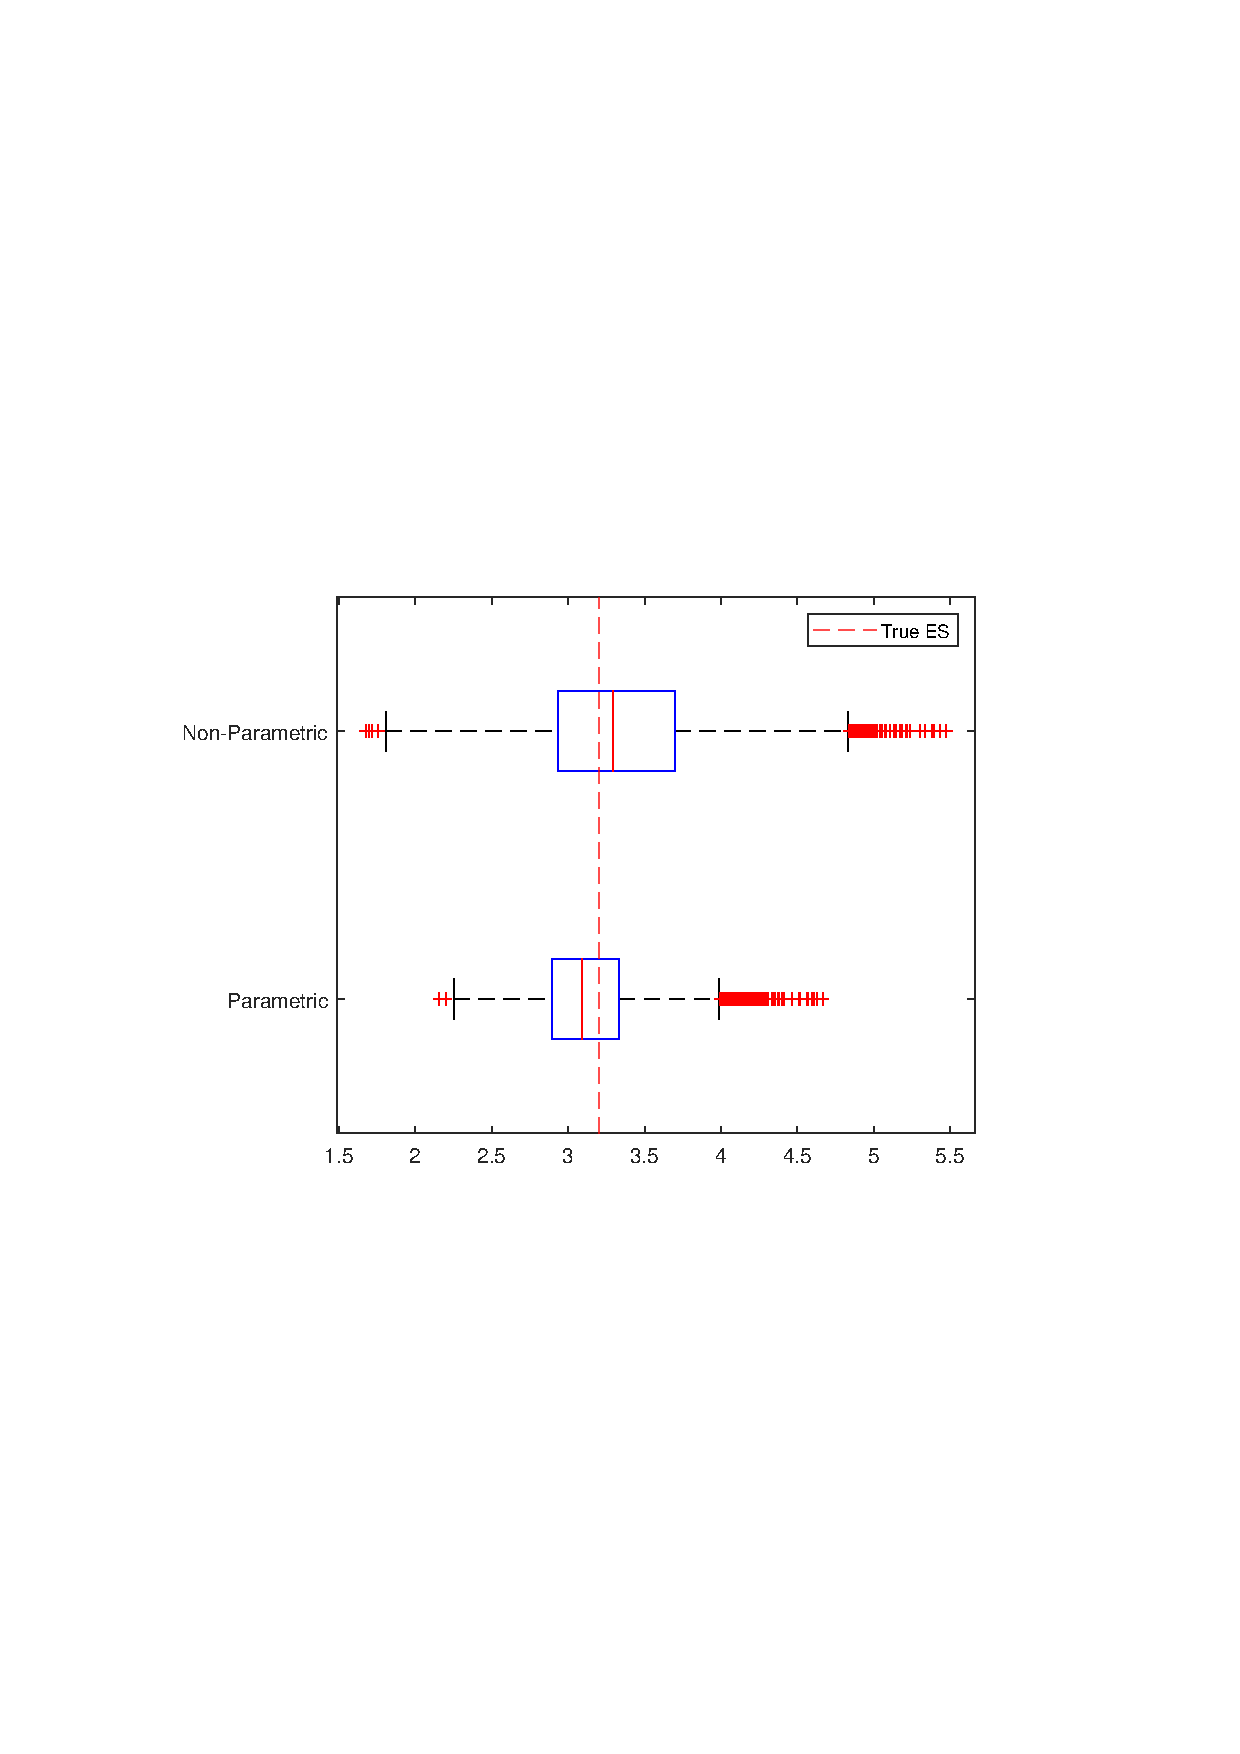
\includegraphics[width=1\linewidth, trim = {0cm 10cm 0cm 10cm}, clip]{boxplot_df4_n250_10000_0.05}
		\end{tabular}
		\caption{\footnotesize Boxplots for ES\textsubscript{5\%} with $df=4$ $n=250$ and $B=10000$.}
		\label{fig1}
	\end{figure}

Figures \ref{fig2a} and \ref{fig2b} show the histograms of the bootstrapped samples for both parametric and non-parametric methods for $n=250$, $B=10000$ and ES\textsubscript{5\%}. The difference in dispersion in both plots reflects the increased uncertainty associated with the non-parametric method.

	\begin{figure}[!htb]
		\centering 
		\begin{subfigure}{.4\linewidth}
			\centering
			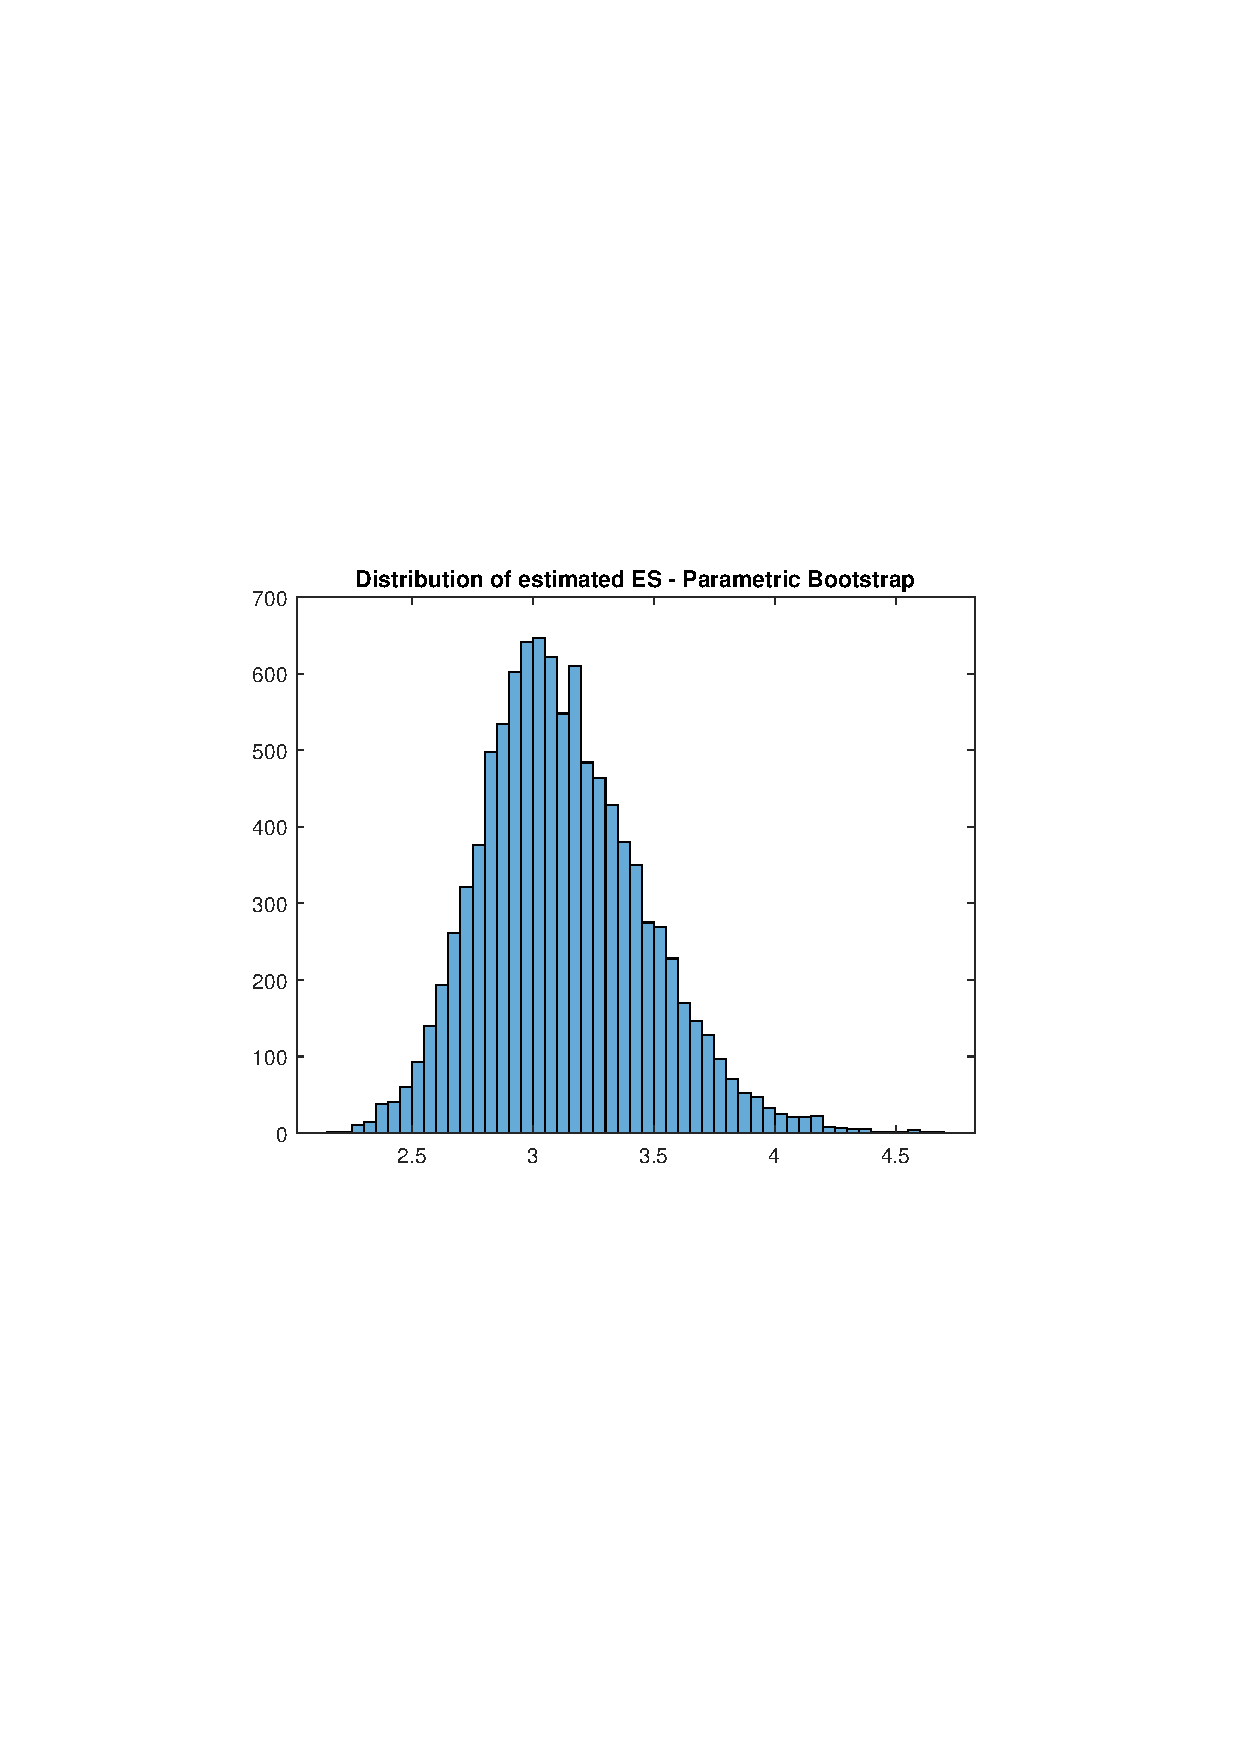
\includegraphics[width=1\linewidth, trim = {0cm 10cm 0cm 10cm}, clip]{parametric_df4_n250_10000_0.05}
		\caption{\footnotesize Paramatric Bootstrap. }
		\label{fig2a}
		\end{subfigure} %
		\begin{subfigure}{.4\linewidth}
			\centering
			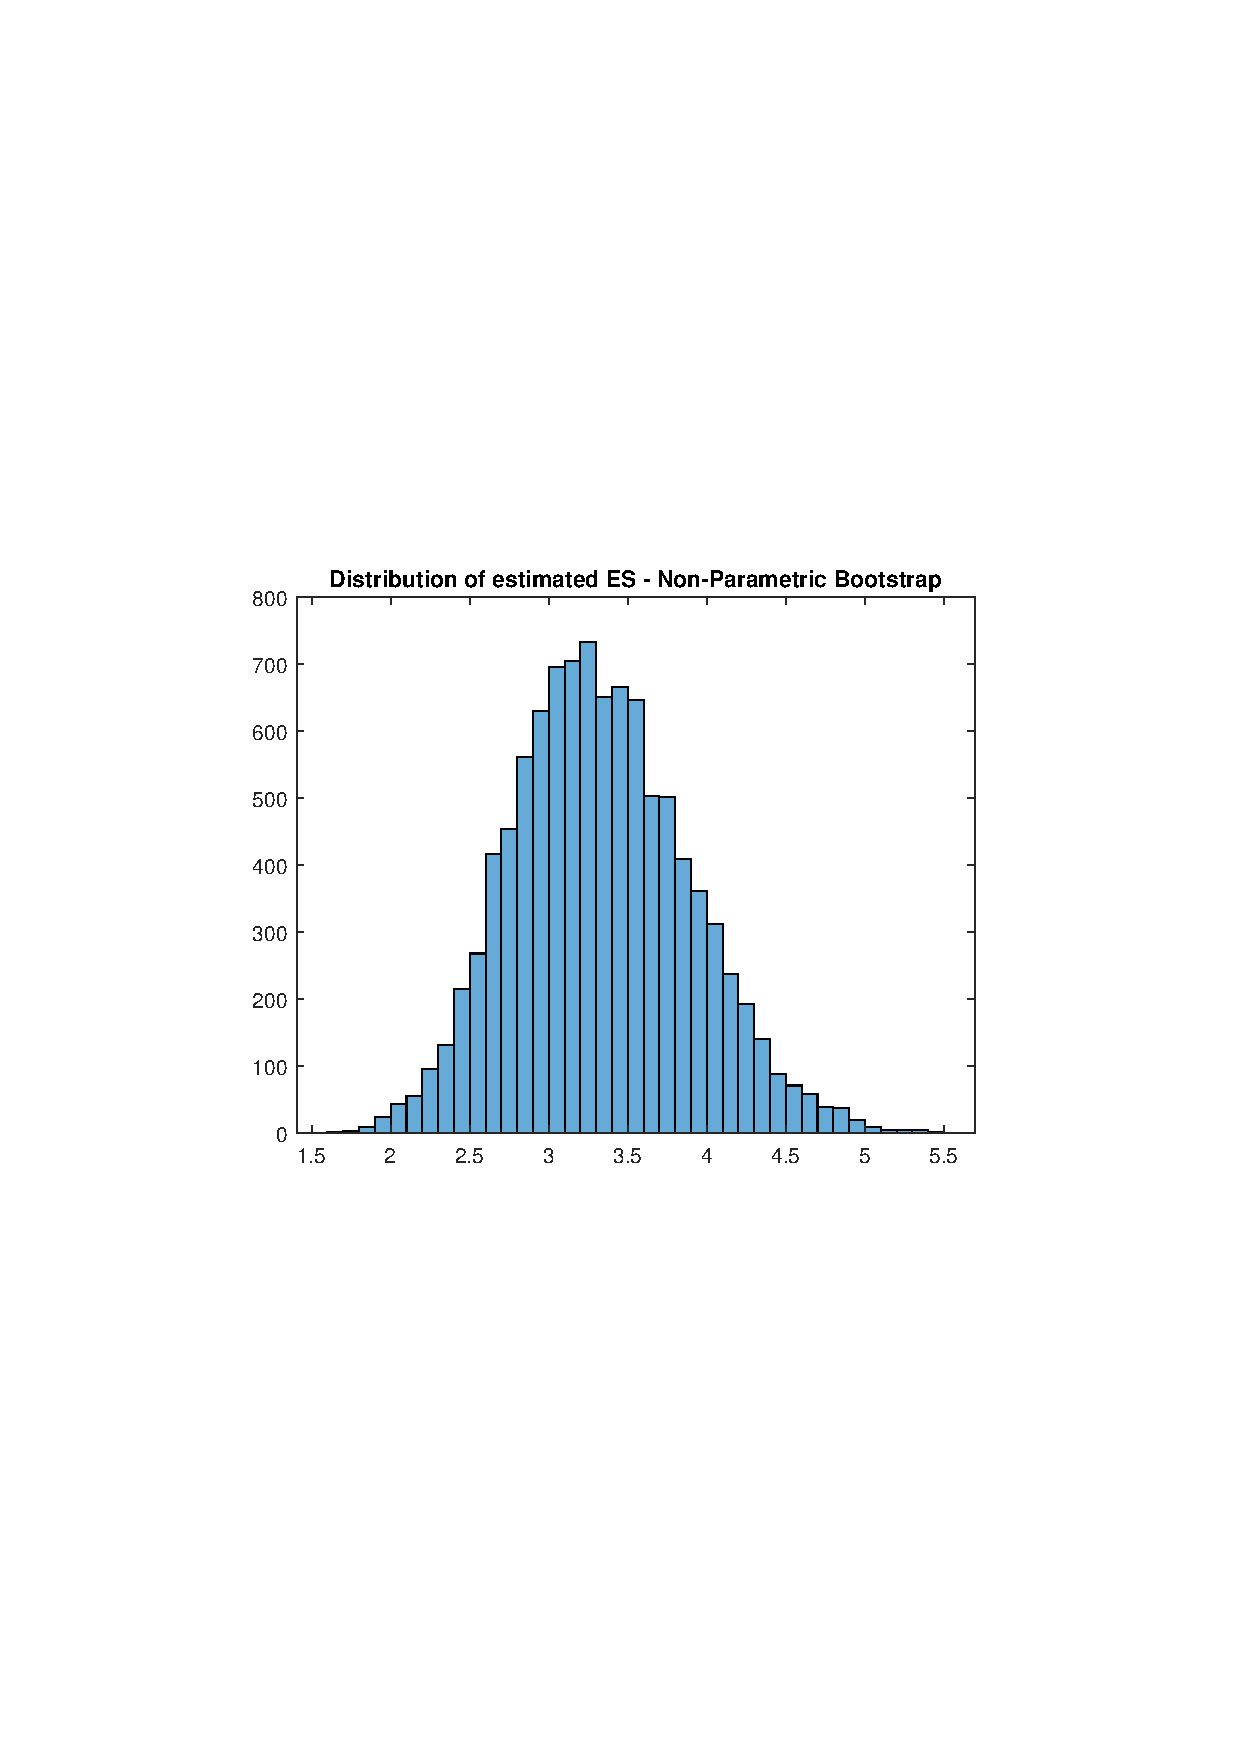
\includegraphics[width=1\linewidth, trim =  {0cm 10cm 0cm 10cm}, clip]{non_parametric_df4_n250_10000_0.05}
			\caption{\footnotesize Non-parametric Bootstrap.}
			\label{fig2b}
		\end{subfigure}
		\caption{\footnotesize ES\textsubscript{5\%} with $df=3$ $n=250$ and $B=5000$.}
		\label{fig2}
	\end{figure}


Both Figures \ref{fig2a} and \ref{fig2b} display a bell-shaped distribution, but this outcome changes significantly for the non-parametric bootstrap when working with ES\textsubscript{1\%} instead of ES\textsubscript{5\%}. This is due to the small sample size. For $n=250$, we have few tail events in our sample. The scarcity of samples deep into the tails translates into more difficult inference for lower ES Levels, particularly for the non-parametric method. Since we resample with replacement in this case, the tail events that could manifest in our bootstrapped samples are limited to the ones we actually observed. Since tail events are rarer, the consequence is that for lower ES levels, the histogram of the non-parametric method loses granularity, whereas the parametric one preserves the bell-shaped appearance. This is best illustrated in Figures \ref{fig3}, \ref{fig4a} and \ref{fig4b}.\\


	\begin{figure}[!htb]\center 
		\begin{tabular}{c}
			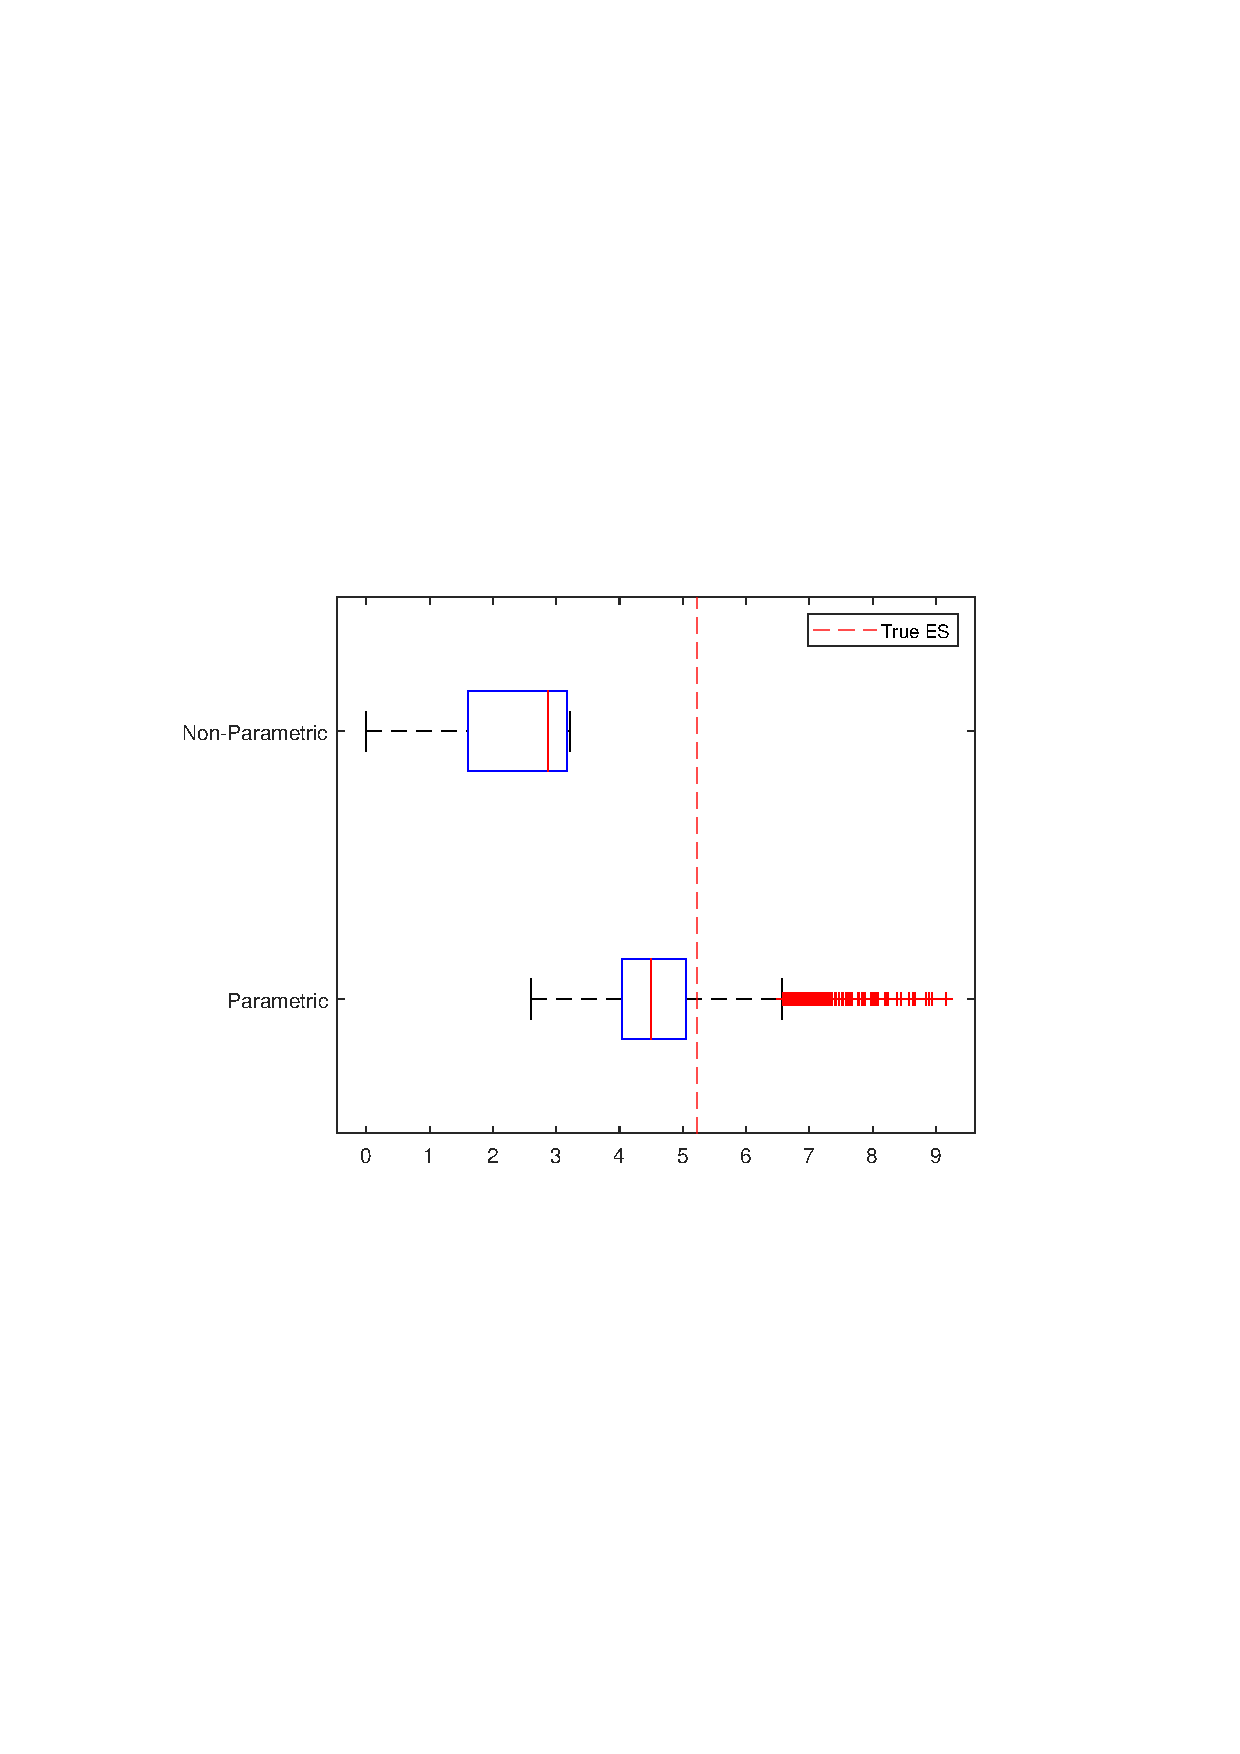
\includegraphics[width=1\linewidth, trim = {0cm 10cm 0cm 10cm}, clip]{boxplot_df4_n250_10000_0.01}
		\end{tabular}
		\caption{\footnotesize Boxplots for ES\textsubscript{1\%} with $df=4$ $n=250$ and $B=10000$.}
		\label{fig3}
	\end{figure}

	\begin{figure}
		\centering 
		\begin{subfigure}{.4\linewidth}
			\centering
			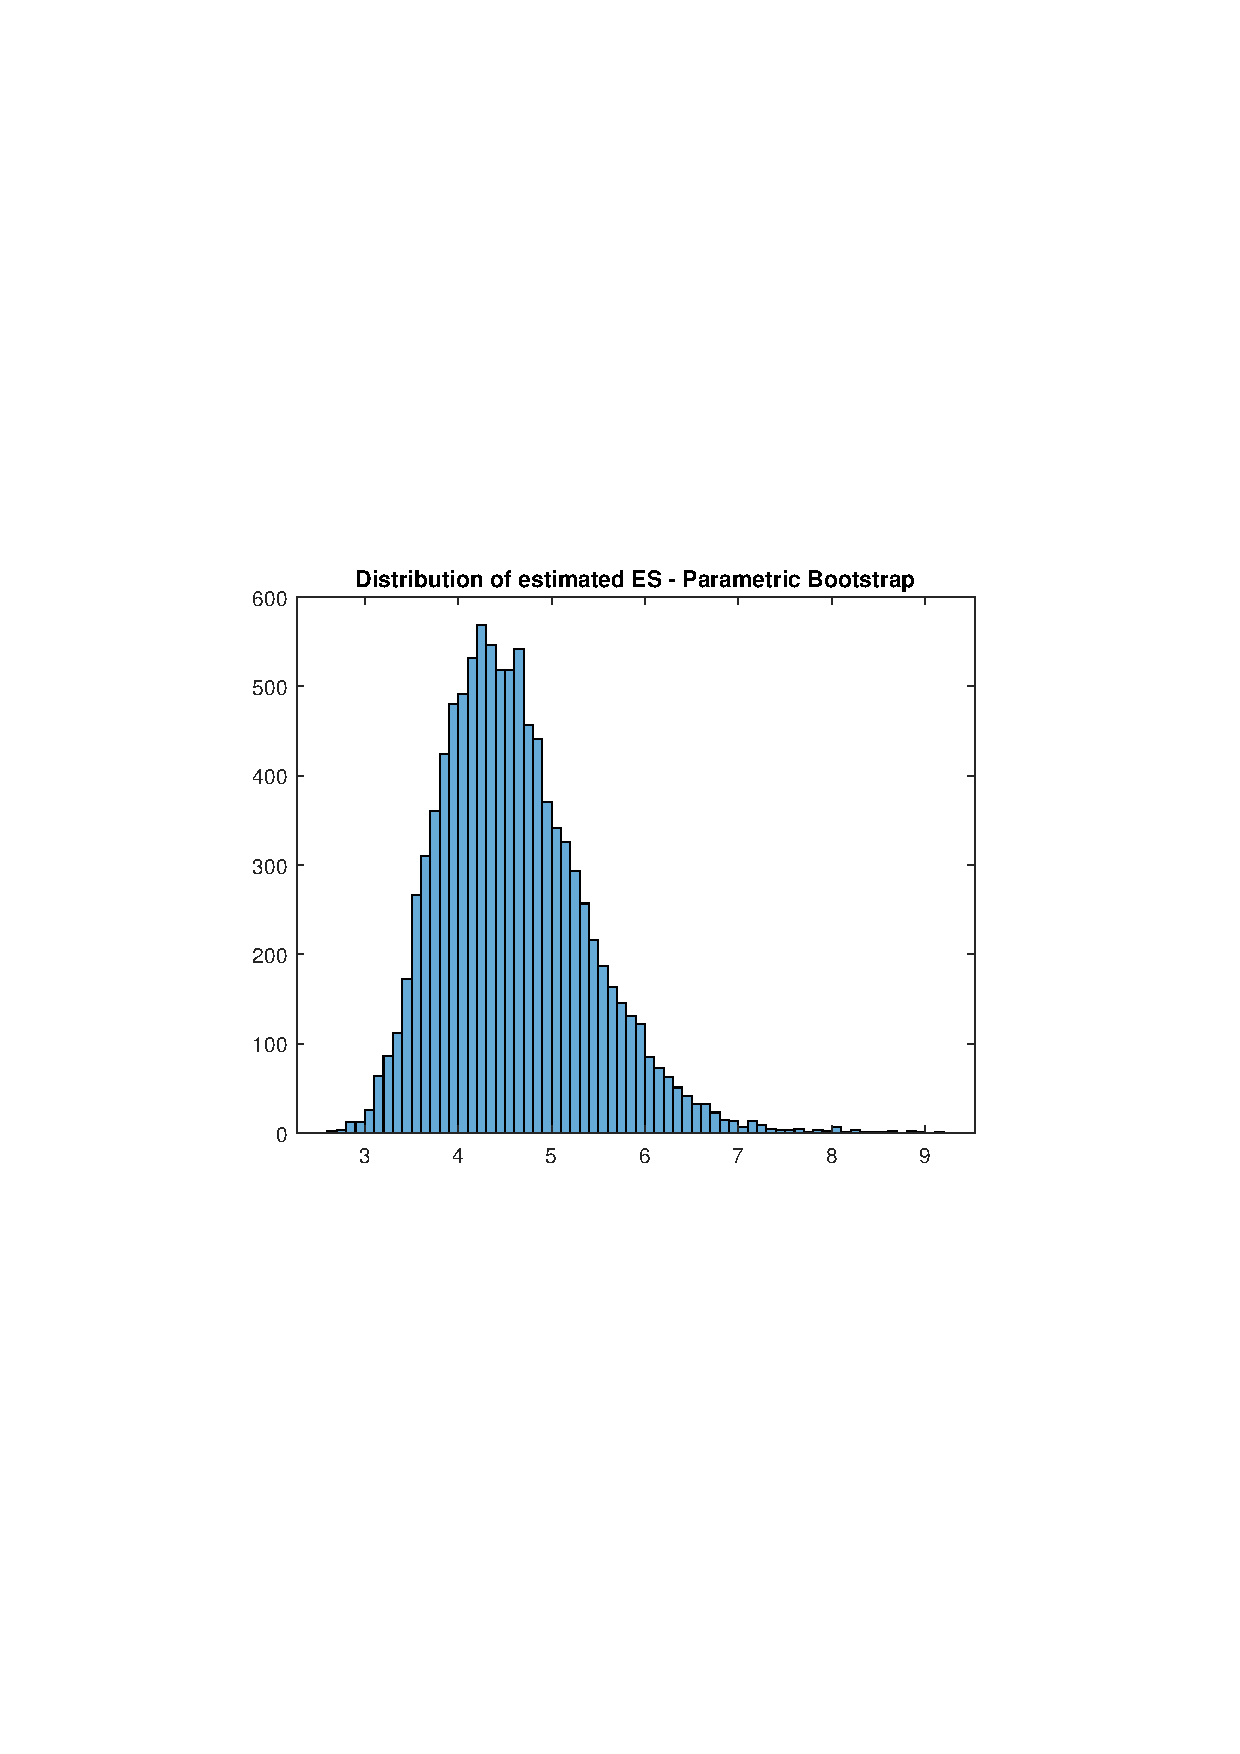
\includegraphics[width=1\linewidth, trim = {0cm 10cm 0cm 10cm}, clip]{parametric_df4_n250_10000_0.01}
		\caption{\footnotesize Paramatric Bootstrap.}
		\label{fig4a}
		\end{subfigure} %
		\begin{subfigure}{.4\linewidth}
			\centering
			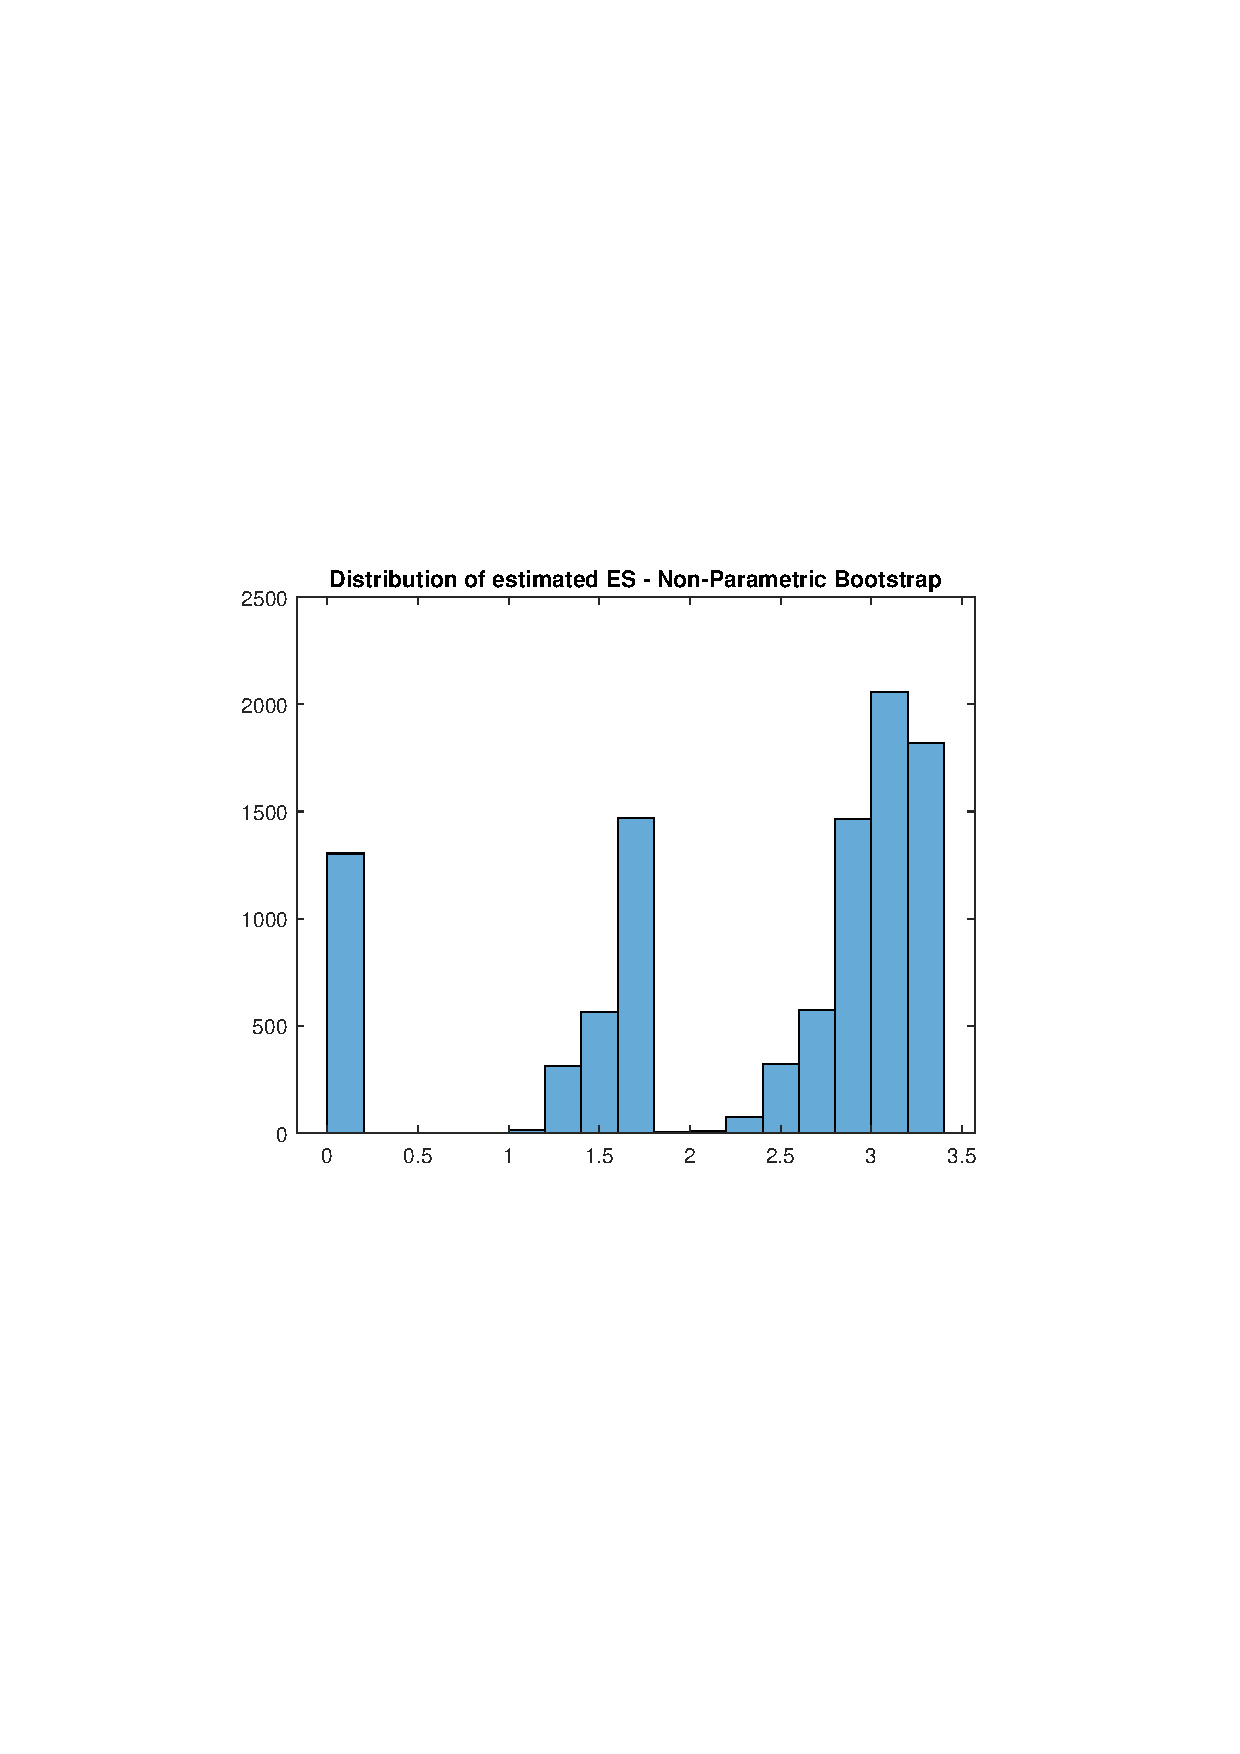
\includegraphics[width=1\linewidth, trim =  {0cm 10cm 0cm 10cm}, clip]{non_parametric_df4_n250_10000_0.01}
			\caption{\footnotesize Non-parametric Bootstrap.}
			\label{fig4b}
		\end{subfigure}
		\caption{\footnotesize ES\textsubscript{1\%} with $df=4$ $n=250$ and $B=10000$.}
		\label{fig4}
	\end{figure}

This issue can be addressed with a larger sample size, since the number of tail events then becomes reasonably large again. Figures \ref{fig7a} and \ref{fig7b} depict the histograms for both methods when $n=25000$. Unfortunately, in practice, obtaining a higher sample size is not always feasible.

	\begin{figure}[!htb]
		\centering 
		\begin{subfigure}{.4\linewidth}
			\centering
			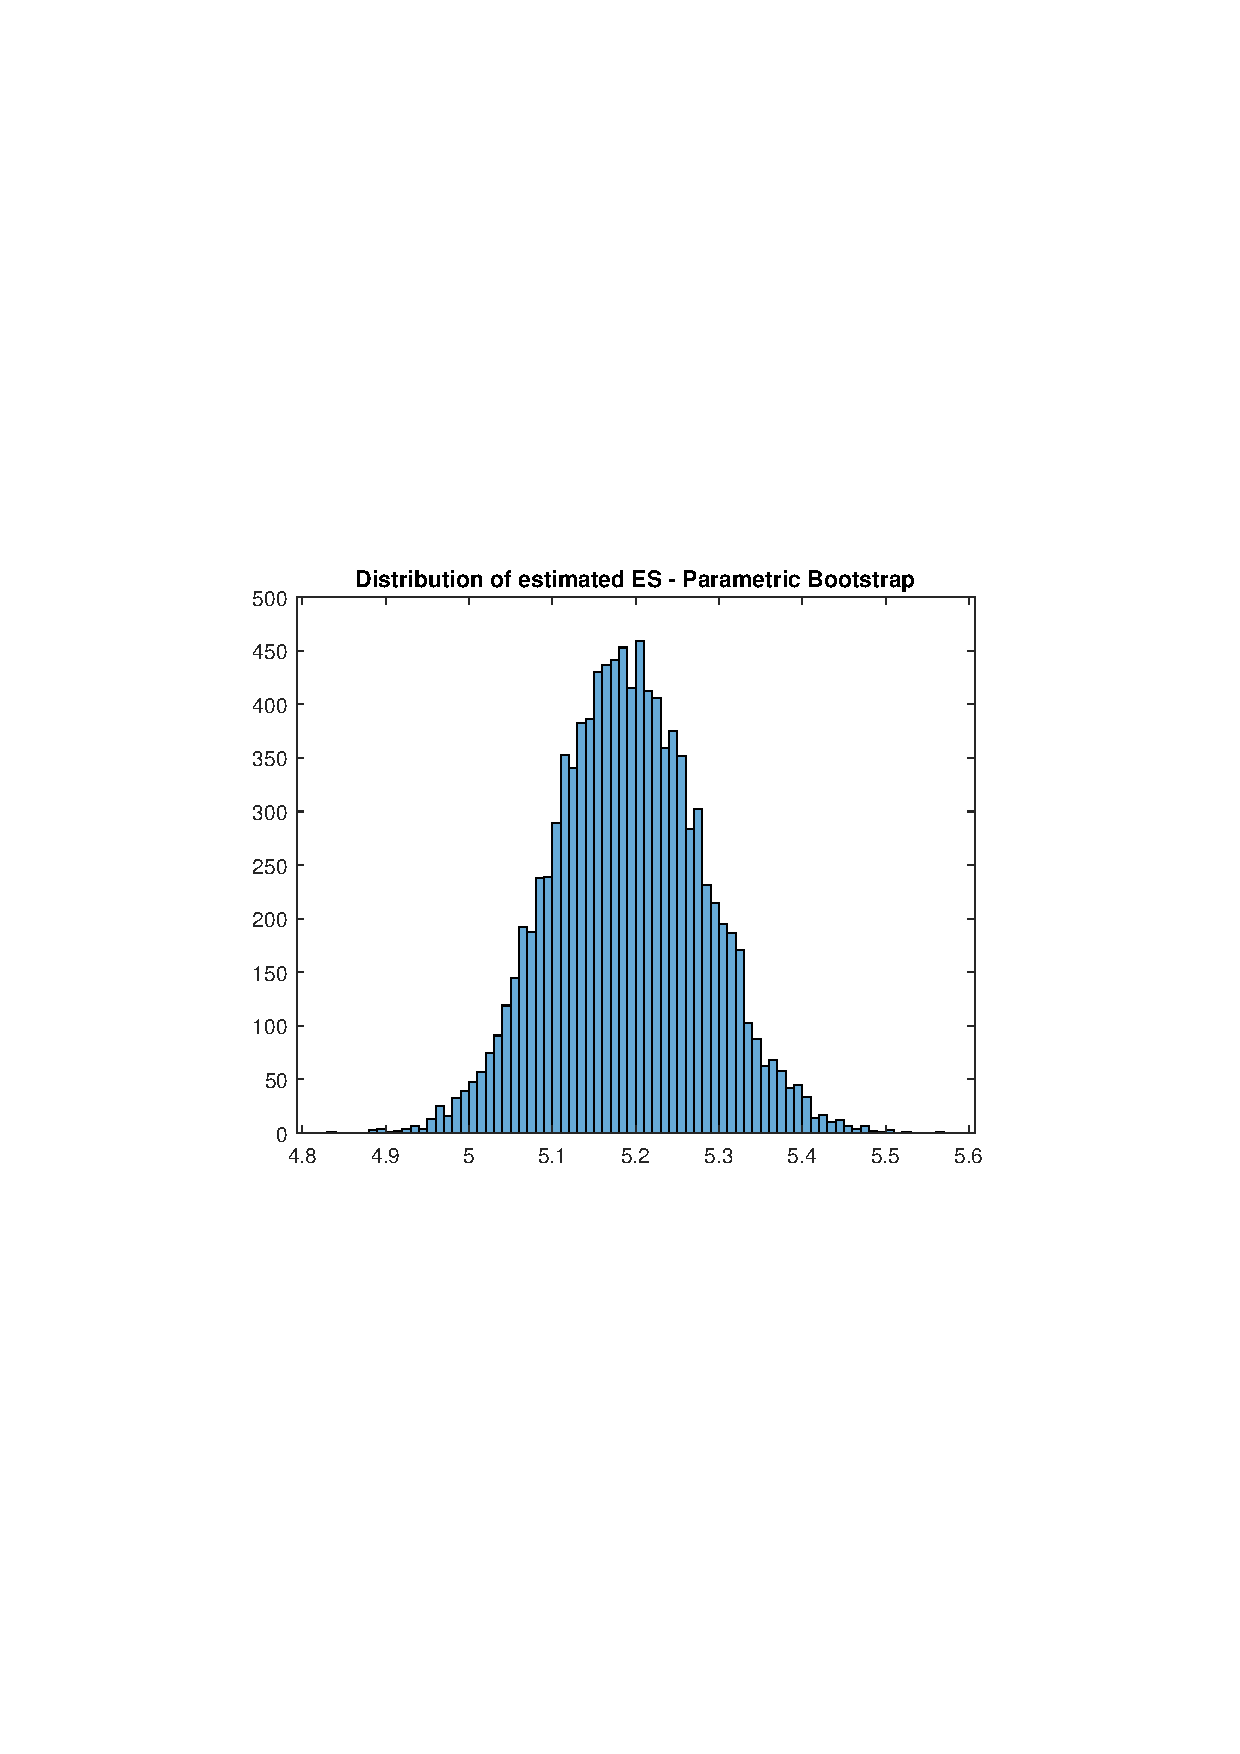
\includegraphics[width=1\linewidth, trim = {0cm 10cm 0cm 10cm}, clip]{parametric_df4_n25000_10000_0.01}
		\caption{\footnotesize Paramatric Bootstrap.}
		\label{fig7a}
		\end{subfigure} %
		\begin{subfigure}{.4\linewidth}
			\centering
			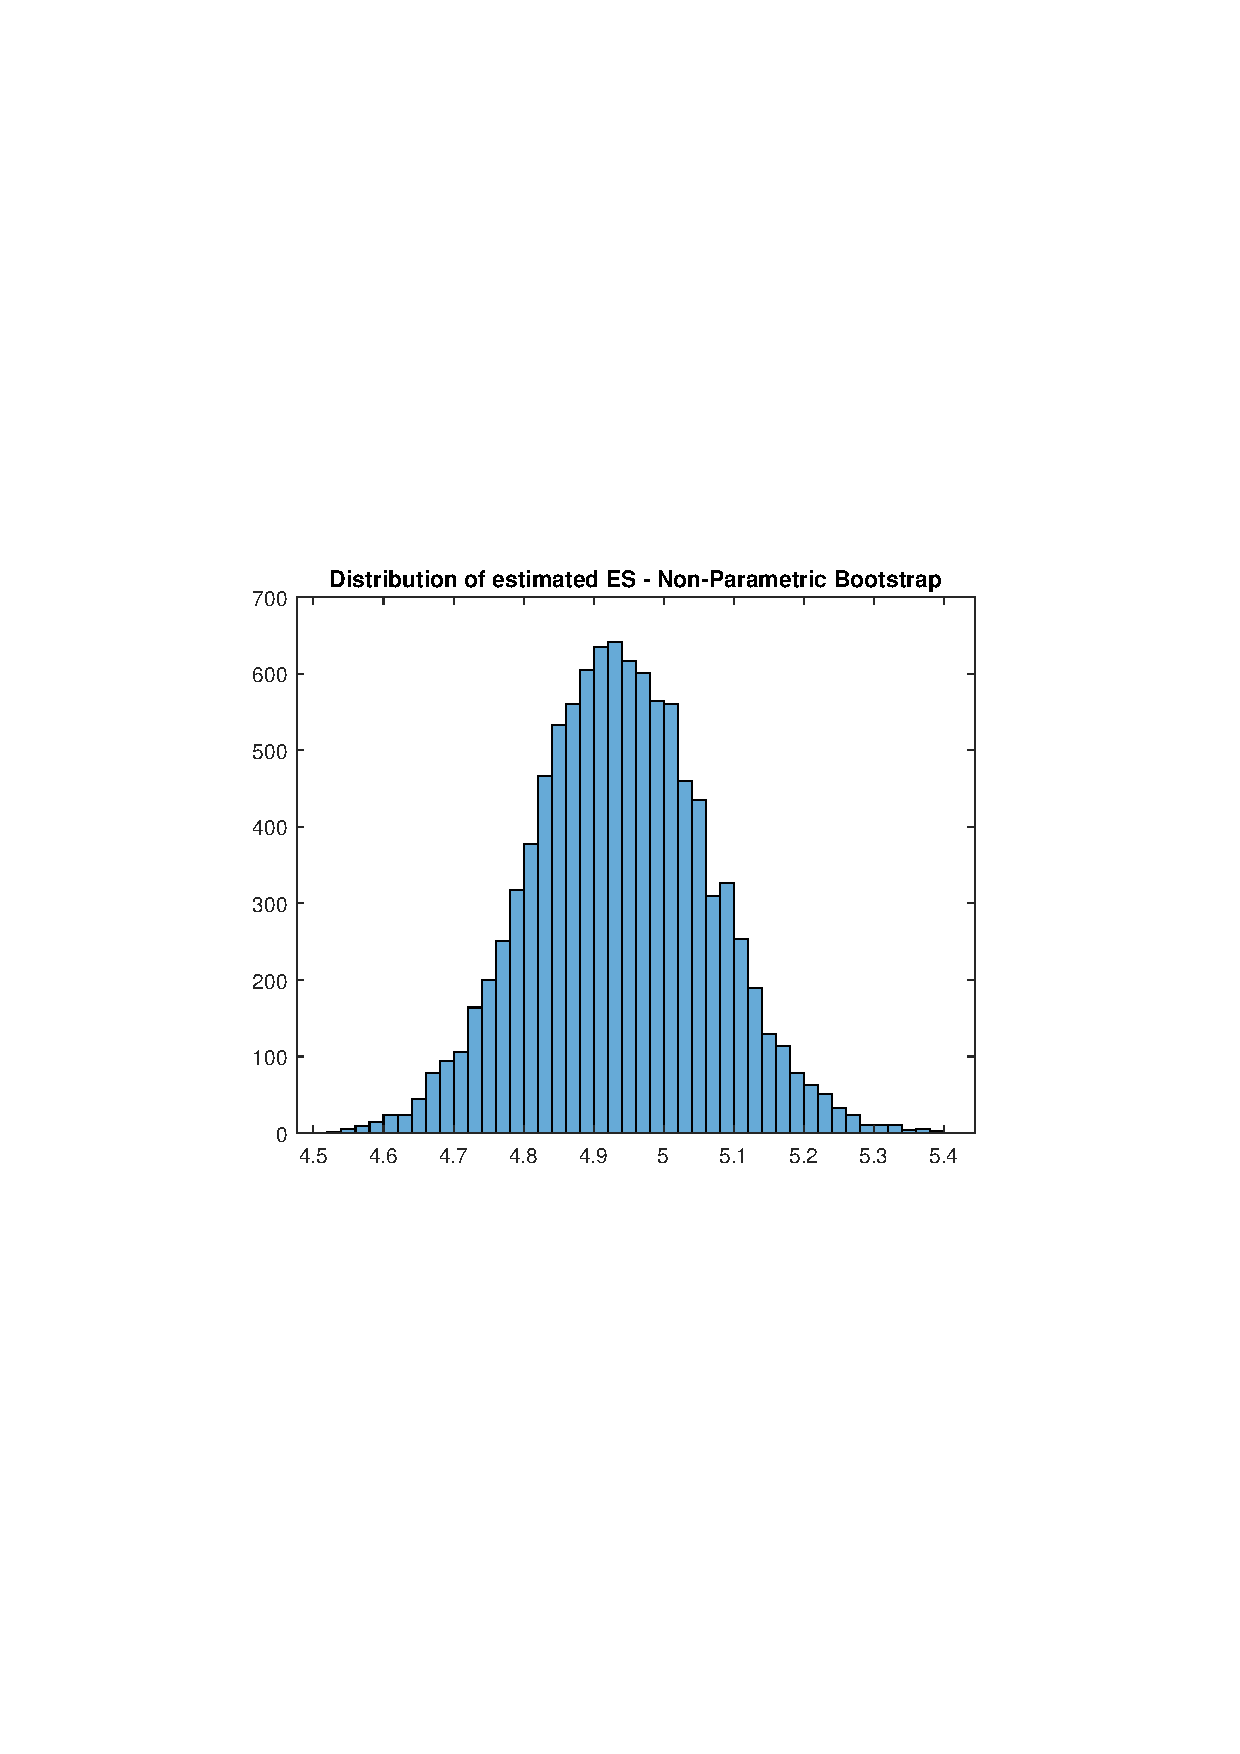
\includegraphics[width=1\linewidth, trim =  {0cm 10cm 0cm 10cm}, clip]{non_parametric_df4_n25000_10000_0.01}
			\caption{\footnotesize Non-parametric Bootstrap.}
			\label{fig7b}
		\end{subfigure}
		\caption{\footnotesize ES\textsubscript{1\%} with $df=4$ $n=25000$ and $B=10000$.}
		\label{fig7}
	\end{figure}


\section{Simulating the Simulation}
In order to check if our CI does its job, meaning that e.g. a 90\% CI captures the true ES 90\% of the time, we add another layer of simulation on top of our bootstrap method. The function coverage\_ES() calls the procedure described above $sim$ number of times and records for each run whether the reported Confidence Intervals actually capture the true ES. The actual coverage is then given by the mean of the output vector. Ideally, the nominal coverage, specified as $confidence\_level$ in the code, should equal the actual coverage, as obtained by simulating the bootstrap method. If the actual coverage is below the nominal coverage, we haven't captured the true ES often enough, meaning that our CI was too narrow.\\

In addition, for each run the length of the CI is stored and again its mean is reported. Comparing the average length of the CI gives a sense of which method performs better.\\

\begin{lstlisting}[style=Matlab-editor]
parfor k = 1 : sim

	[trueES, ~, IC_parametric, ~, IC_nonparametric]  = ES_bootstrap(df, n, B, ESlevel, location, scale);
	is_in_interval_par(k, 1) = (trueES >= IC_parametric(1) && trueES <= IC_parametric(2));
	is_in_interval_nonpar(k, 1) = (trueES >= IC_nonparametric(1) && trueES <= IC_nonparametric(2));       
	interval_length_par(k, 1) = IC_parametric(2) - IC_parametric(1);
	interval_length_nonpar(k, 1) = IC_nonparametric(2) - IC_nonparametric(1);

end

is_in_interval = [is_in_interval_par , is_in_interval_nonpar];
interval_length = [interval_length_par, interval_length_nonpar];

mean(is_in_interval)
mean(interval_length)
\end{lstlisting}
\label{Coverage function}
\captionof{lstlisting}[matlab2]{Obtain the actual coveraga based on $sim$ number of simulations\\}

A particular feature of this function is that we implemented it using a PARFOR loop, which in Matlab allows for faster computation of the simulations by parallelizing the work. In our tests, running the coverage\_ES() function with  $sim = 1000$, $B = 500$ and $n = 250$ with the paralell loop takes about 5 minutes.\\

\subsection{The effects of the shape parameter}
We also wanted to verify how the actual CI coverage and CI length change for different degrees of freedom. In order to do this, we looped the coverage\_ES() function for multiple degrees of freedom ranging from 2 to 10 for an ES level of 5\%, and 90\% nominal CI. This procedure was computationally intensive and required around three hours of run time. \\

From the plot below, it is possible to see that the parametric bootstrap performs quite well, achieving actual coverage ratios greater than 85\% for all df's for a nominal 90\% CI. It is also possible to see that the CI is biased negatively, as the actual coverage never really reaches 90\%. \\

	\begin{figure}[!htb]\center 
		\begin{tabular}{c}
			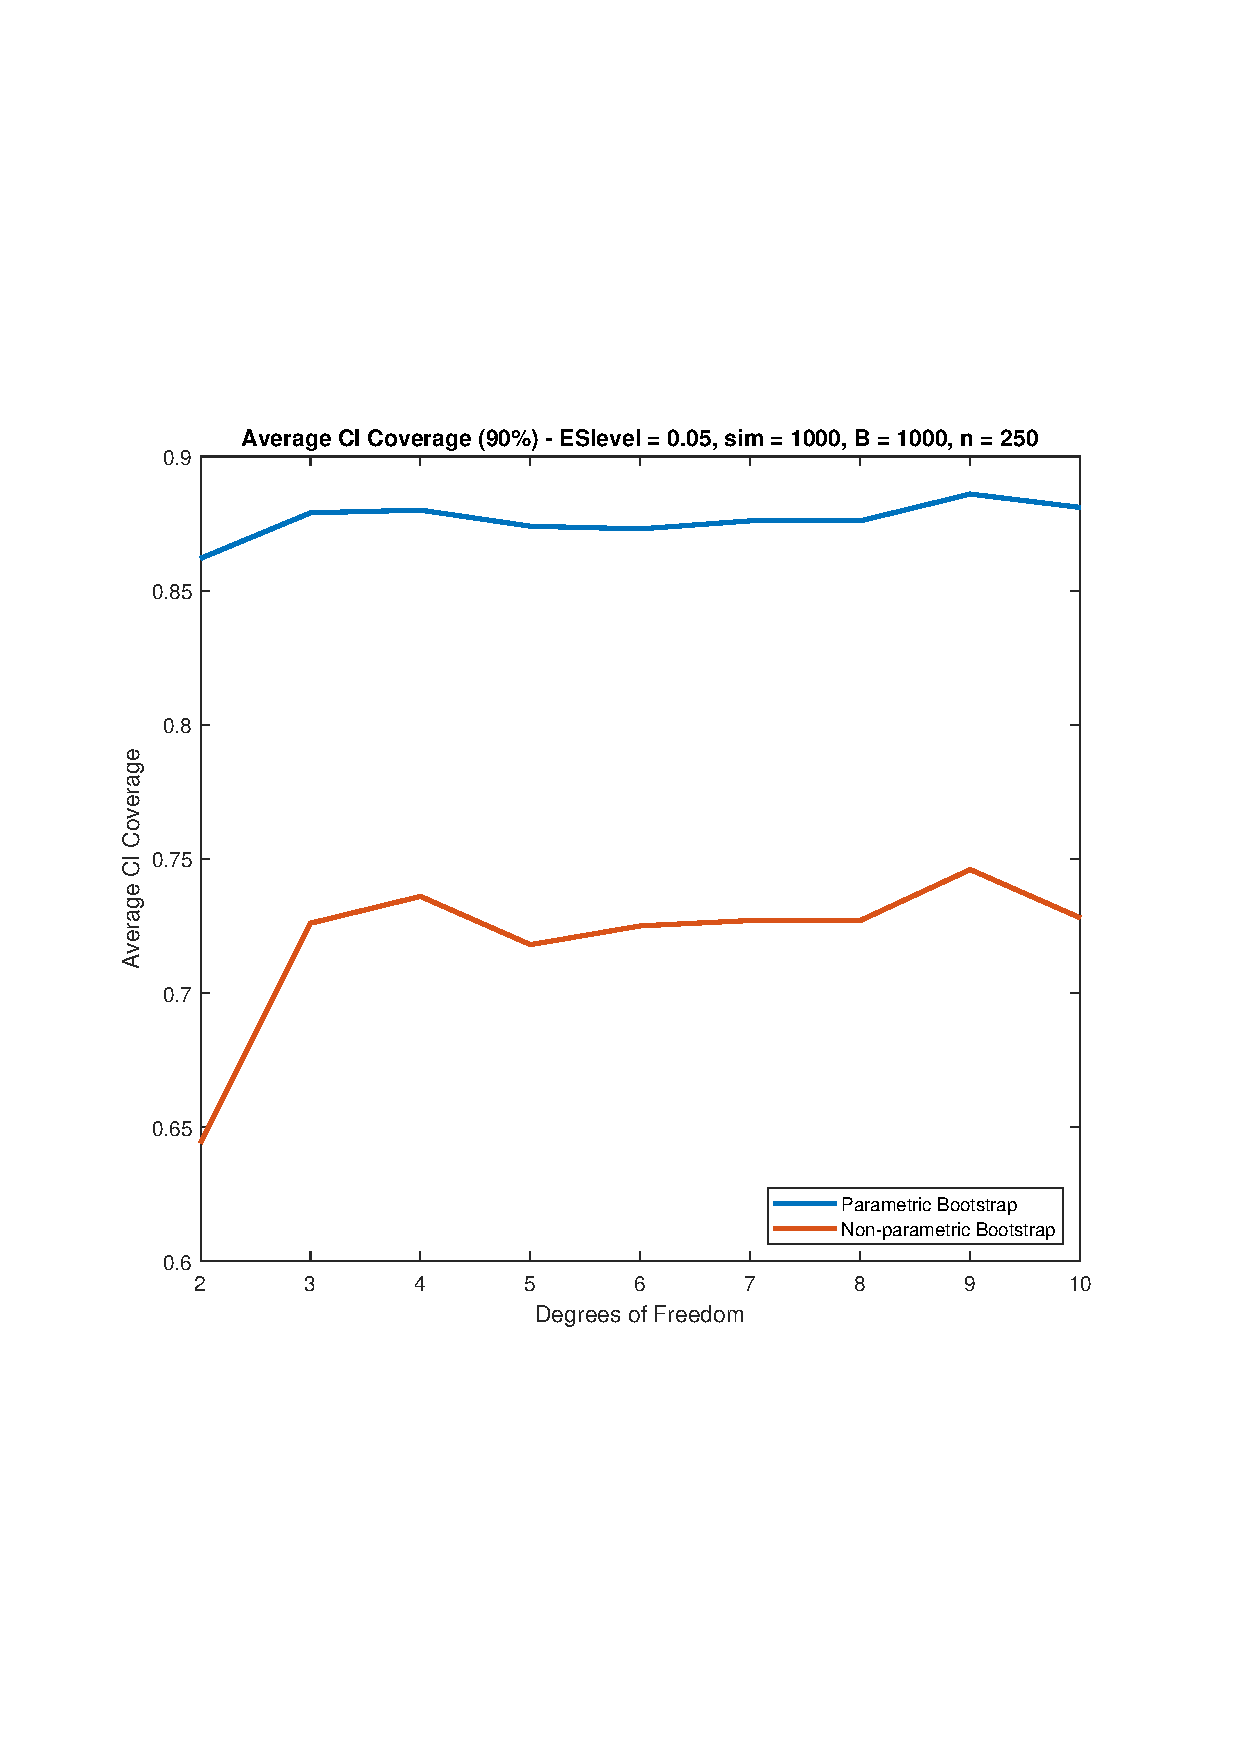
\includegraphics[width=1\linewidth, trim =  {0cm 7cm 0cm 7cm}, clip, scale =0.75]{avg_coverage_x_dfs.pdf}
		\end{tabular}
		\caption{\footnotesize Actual coverage for parametric and non-parametric bootstraps.}
		\label{fig8}
	\end{figure}

	\begin{figure}[!htb]\center 
		\begin{tabular}{c}
			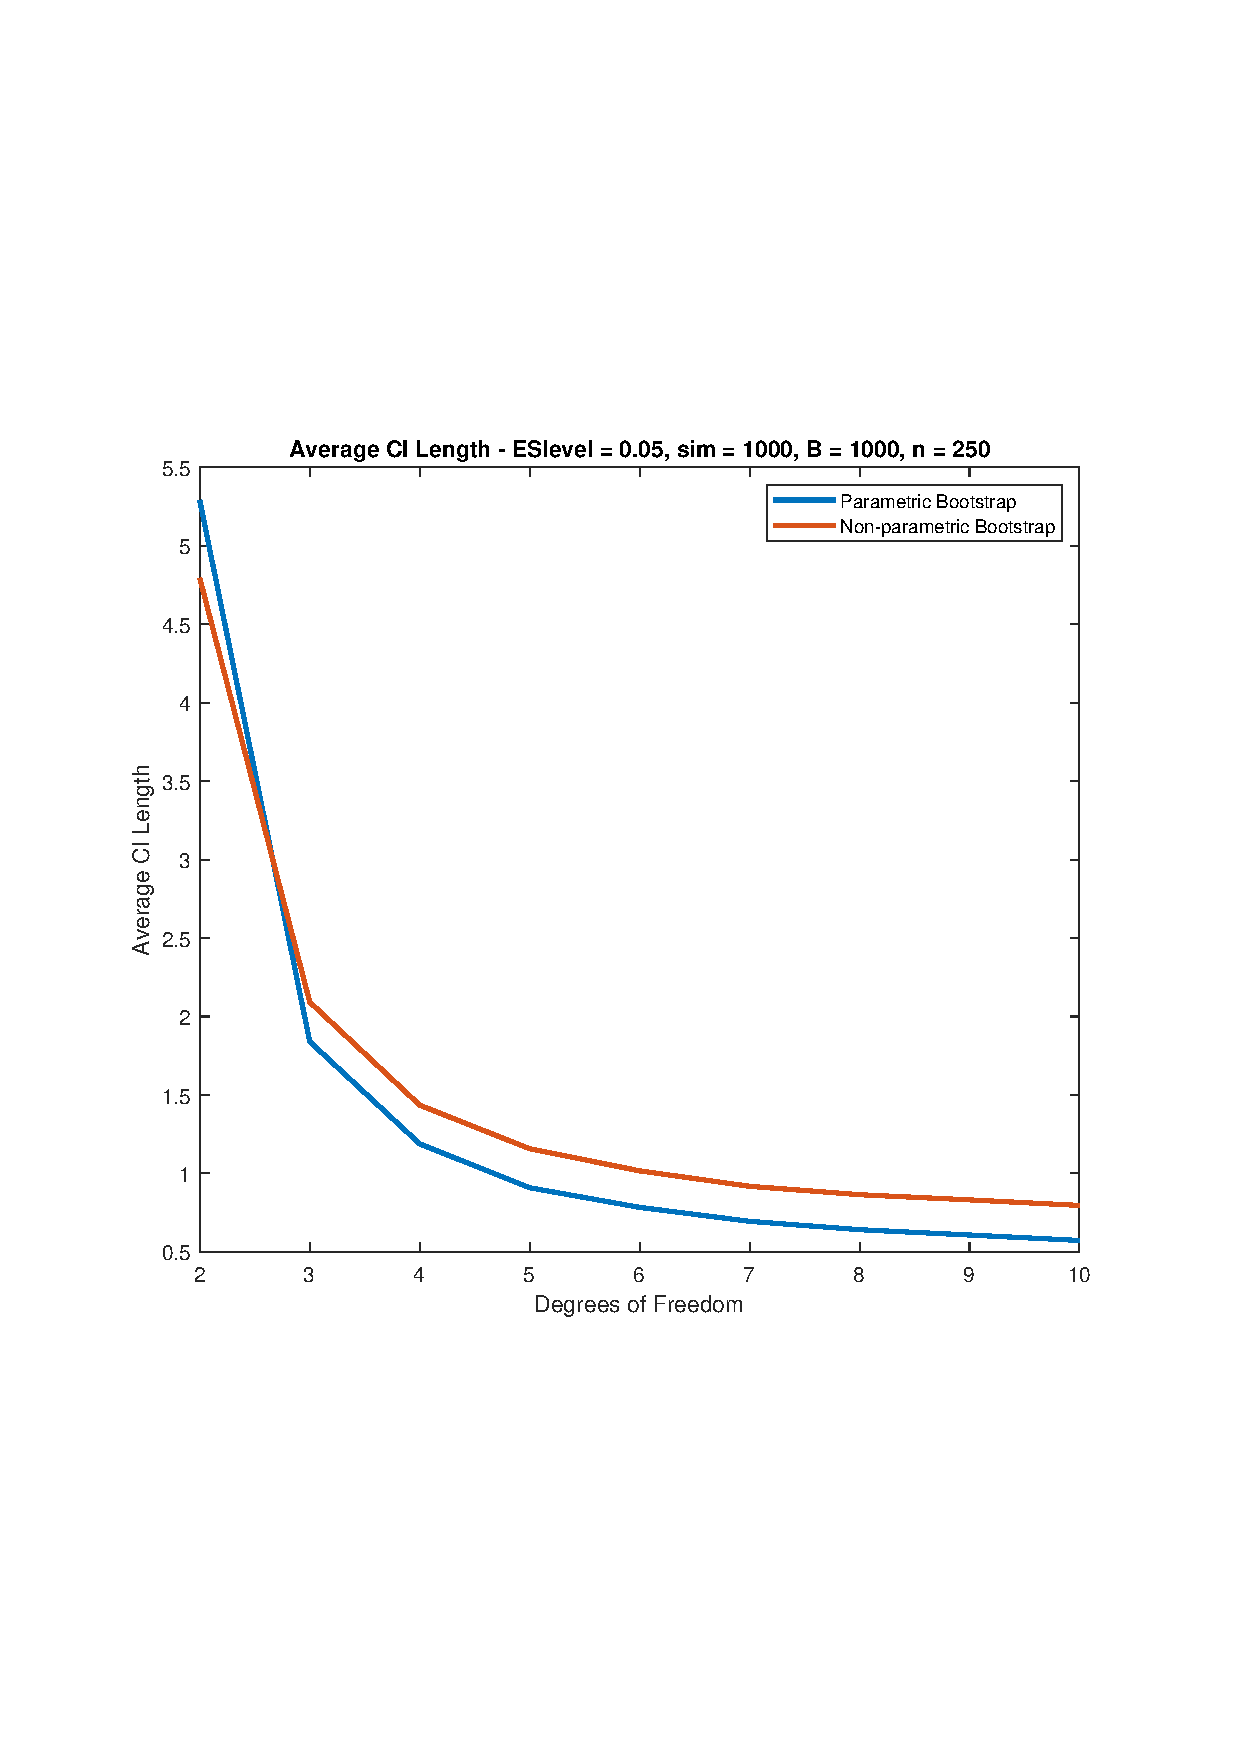
\includegraphics[width=1\linewidth, trim = {0cm 7cm 0cm 7cm}, clip, scale = 0.75]{avg_length_x_dfs.pdf}
		\end{tabular}
		\caption{\footnotesize Average CI length for parametric and non-parametric bootstraps.}
		\label{fig9}
	\end{figure}

For the non-parametric case, however, the bias is more significant, with actual coverage ratios never quite reaching 75\%. The shape parameter doesn't seem to affect the  CI coverage that much, except for very low df's. \\

Figure \ref{fig9} shows the average CI length for different degrees of freedom. Here the impact of fatter tails becomes more evident: as degrees of freedom get smaller, the 90\% nominal CI becomes larger, reflecting the growing uncertainty about the true ES due to the thicker tails. Once more, the parametric bootstrap performs better than the non-parametric version. \\

Interestingly, the non-parametric method produced narrower CI for the df = 2 case, but, as seen from the low actual coverages in Figure \ref{fig8}, it is clear that the non-parametric method is being too liberal. \\

Both of these graphics show how much the extra information used by the Parametric Bootstrap matters when calculating  CI's. However, this is conditional on correctly assuming the underlying distribution and the performance ranking between the two methods may easily switch under bad assumptions.\\

\subsection{Using additional information about the underlying sample distribution}
While in practice we do not have exact details about the parameters of the underlying distribution, let's assume for now that we actually do know some parameters. If we now assume that location and scale parameters are known to be zero and one, respectively, just as the default input arguments of our functions are, we can change the bootstrap procedure to make use of this extra information, and hence expect better performance than the parametric bootstrap method. \\

The mle() function now fits the data to the PDF of a location 0, scale 1 Student's t and hence forces the location-scale parameters to be the exact ones, therefore only uncertainty about the degrees of freedom remains. This Bootstrap method for obtaining a CI for the ES is again repeated $B$ times.\\


\begin{lstlisting}[style=Matlab-editor]
%Alternatively, force location=0, scale=1 and only estimate df
pd_student_t = @(x,df) tpdf(x,df);
paramaters_hat = mle(random_sample, 'pdf' ,pd_student_t,'Start',1);
location_hat = 0;
scale_hat = 1;
df_hat = paramaters_hat(1);
\end{lstlisting}
\label{MLE location 0 scale 1}
\captionof{lstlisting}[matlab2]{Implent the MLE for location 0, scale 1\\}

\begin{lstlisting}[style=Matlab-editor]
for k = 1 : B
	
	parametric_bootstrap_sample = trnd(df_hat, [n, 1]) * scale_hat + location_hat;
	mle_output = mle(parametric_bootstrap_sample, 'pdf' ,pd_student_t,'Start',1);
	
	% The MLE output for the degrees of freedom may be smaller than 1,     
	% for which we don't have a true ES. In this case, we use df = 1.01
	% instead.
	df_input = max(mle_output(1), 1.01);                                        
	ES_param_bootstrap(k, 1) = ES_formula(df_input, ESlevel, 0, 1);
	
end
\end{lstlisting}
\label{MLE location 0 scale 1 bootstrap}
\captionof{lstlisting}[matlab2]{Apply the Bootstrap with location 0, scale 1\\} 


Applying this procedure with the same setting as in figure \ref{fig9} for degrees of freedom 2 and 10, we can see the improvement we get from adding additional information to the bootstrap method. While the actual coverage remained almost the same, since it was already very close to 90\% in the first case, the average length of the CI decreases quite a bit. \\

For 2 df's, we could report an average length of 4.7188 in the case where we made use of the additional information on the parameters, as compared to 5.4282 in the general case. For 10 df's, the average CI length decreased from 0.5743 to 0.5165.

\clearpage
\section{Appendix}
\subsection{True ES - Code}
\begin{lstlisting}[style=Matlab-editor]
function ES = ES_formula(df, ESlevel, location, scale)
   
    %% Veryfing inputs are correct and setting up defaults.
    %(df, ESlevel, location, scale)
    if nargin == 1
        ESlevel = 0.05;
        location = 0;
        scale = 1;
    elseif nargin == 2
        location = 0;
        scale = 1;
    elseif nargin == 3
        scale = 1;
    end
    
    %verify inputs
    if df <= 1
        msgbox('Degrees of freedom must be greater than 1.')
        return
    end
    if ESlevel >= 1 || ESlevel <= 0
        msgbox('Alpha must be between 0 and 1.')
        return
    end
    
    %% True ES
    ES = -location + (1 / (df - 1)) * (scale / ESlevel) * tpdf(tinv(ESlevel, df), df) * (df + tinv(ESlevel, df)^2);
end


\end{lstlisting}
\label{matlab111}
\captionof{lstlisting}[matlab111]{Code for ES\_formula().}

\newpage
\subsection{Parametric and non-parametric Bootstrap - Code}
\begin{lstlisting}[style=Matlab-editor]
function [trueES, ES_hat_parametric, IC_parametric, ES_hat_nonparametric, IC_nonparametric]  = ES_bootstrap(df, n, B, ESlevel, location, scale)
    
    %% TURN OFF MLE WARNING
    warning('off', 'stats:tlsfit:IterLimit')
    %warning('on', 'stats:tlsfit:IterLimit')
    warning('off', 'stats:mlecov:NonPosDefHessian')
    % warning('on', 'stats:mlecov:NonPosDefHessian')
    
    
    %% Veryfing inputs are correct and setting up defaults.
    %(df, n, B, ESlevel, location, scale)
    if nargin == 1
        n = 250;
        B = 500;
        ESlevel = 0.05;
        location = 0;
        scale = 1;
    elseif nargin == 2
        B = 500;
        ESlevel = 0.05;
        location = 0;
        scale = 1;
    elseif nargin == 3
        ESlevel = 0.05;
        location = 0;
        scale = 1;
    elseif nargin == 4
        location = 0;
        scale = 1;
    elseif nargin == 5
        scale = 1;
    end

    %verify inputs
    if df <= 1
        msgbox('Degrees of freedom must be greater than 1.')
        return
    end
    if ESlevel >= 1 || ESlevel <= 0
        msgbox('ESlevel must be between 0 and 1.')
        return
    end
    if n <= 0 || B <= 0
        msgbox('n and B must be greater than zero')
        return
    end
    
    %% Configuration of confidence interval
    confidence_level = 0.9;
    alpha = 1 - confidence_level;
    
    %% Generate the random iid sample:
    random_sample = scale * trnd(df, [n, 1]) + location;
    
    %% True ES by calling the true_ES function:
    trueES = ES_formula(df, ESlevel, location, scale);
    
    %% Parametric Bootstrap:
    % First, uses the random_sample to estimate the parameters of the
    % underlying t distribution:
    paramaters_hat = mle(random_sample, 'Distribution' ,'tLocationScale');
    location_hat = paramaters_hat(1);
    scale_hat = paramaters_hat(2);
    df_hat = paramaters_hat(3);
    
    % Second, use the above estimated parameters to calculate the corresponding ES:
        % The MLE output for the degrees of freedom may be smaller than 1,     
        % for which we don't have a true ES. In this case, we use df = 1.01
        % instead.
        df_hat = max(df_hat, 1.01); 
    
    ES_hat_parametric = ES_formula(df_hat, ESlevel, location_hat, scale_hat);
    
    % Third, FOR loop over B, recreating bootstrap samples out of the
    % estimated parameters above and calculating ES via the parametric formula. 
    ES_param_bootstrap = zeros(B, 1);
    
    for k = 1 : B
        parametric_bootstrap_sample = trnd(df_hat, [n, 1]) * scale_hat + location_hat;
        mle_output = mle(parametric_bootstrap_sample, 'Distribution', 'tLocationScale');
        
        
        % The MLE output for the degrees of freedom may be smaller than 1,     
        % for which we don't have a true ES. In this case, we use df = 1.01
        % instead.
        df_input = max(mle_output(3), 1.01);                                        
        ES_param_bootstrap(k, 1) = ES_formula(df_input, ESlevel, mle_output(1), mle_output(2));
    end
    
    % Vector ES_param_bootstrap now contains B estimates of ES calculated with
    % the parametric formula. In order to obtain a confidence interval of 90%, we just
    % need to take the 5%-quantile and the 95%-quantile:
    IC_parametric = quantile(ES_param_bootstrap, [alpha/2, 1 - alpha/2]);
    
    % Last, plot a histogram:
    histogram(ES_param_bootstrap)
    title('Distribution of estimated ES - Parametric Bootstrap')
    
    %% Non-parametric Bootstrap:
    % First, starting from the random sample, calculate the empirical VaR:
    empirical_VaR = - quantile(random_sample, ESlevel);
    
    % Second, calculate the average of the sample tha realized below the
    % empirical_VaR:
    I =(random_sample < - empirical_VaR);
    ES_hat_nonparametric =  - mean(random_sample .* I) / ESlevel;
    
    % Third, FOR loop where we resample with replacemente from the original
    % sample. For each bootstrap sample, calculate the empirical ES and store
    % it:
    ES_nonparam_bootstrap = zeros(B, 1);
    
    for k = 1 : B
        nonparametric_bootstrap_sample = randsample(random_sample, n, true);
        noonparametric_bootstrap_sample_empirical_VaR = - quantile(nonparametric_bootstrap_sample, ESlevel);
        I =(nonparametric_bootstrap_sample < - noonparametric_bootstrap_sample_empirical_VaR);
        ES_nonparam_bootstrap(k, 1) =  - mean(nonparametric_bootstrap_sample .* I) / ESlevel;
    end
    
    % Vector ES_nonparam_bootstrap now contains B estimates of ES calculated
    % via quantile of the bootsrtrap resamples. In order to obtain a confidence 
    % interval of 90%, we just need to take the 5%-quantile and the 95%-quantile:
    IC_nonparametric = quantile(ES_nonparam_bootstrap, [alpha/2, 1 - alpha/2]);
    
    % Last, plot a histogtam
    figure
    histogram(ES_nonparam_bootstrap)
    title('Distribution of estimated ES - Non-Parametric Bootstrap')
    
    %% Summarizing the two results:
    figure
    boxplot([ES_param_bootstrap, ES_nonparam_bootstrap], 'orientation', 'horizontal', 'Labels', {'Parametric', 'Non-Parametric'})
    xline(trueES, 'r--'), legend('True ES')

end

\end{lstlisting}
\label{matlab2}
\captionof{lstlisting}[matlab2]{Code for ES\_bootstrap().}

\newpage
\subsection{CI Coverage - Code}
\begin{lstlisting}[style=Matlab-editor]
function [is_in_interval, interval_length] = coverage_ES(sim, df, n, B, ESlevel, location, scale)
    
    %% Veryfing inputs are correct and setting up defaults.
    %(df, n, B, ESlevel, location, scale)
    if nargin == 2
        n = 250;
        B = 500;
        ESlevel = 0.05;
        location = 0;
        scale = 1;
    elseif nargin == 3
        B = 500;
        ESlevel = 0.05;
        location = 0;
        scale = 1;
    elseif nargin == 4
        ESlevel = 0.05;
        location = 0;
        scale = 1;
    elseif nargin == 5
        location = 0;
        scale = 1;
    elseif nargin == 6
        scale = 1;
    end

    %verify inputs
    if df <= 1
        msgbox('Degrees of freedom must be greater than 1.')
        return
    end
    if ESlevel >= 1 || ESlevel <= 0
        msgbox('ESlevel must be between 0 and 1.')
        return
    end
    if n <= 0 || B <= 0
        msgbox('n and B must be greater than zero')
        return
    end

    % THE CODE BELOW MAKES USE OF PARALLEL COMPUTING
    
    is_in_interval_par = zeros([sim, 1]);
    is_in_interval_nonpar = zeros([sim, 1]);
    interval_length_par = zeros([sim, 1]);
    interval_length_nonpar = zeros([sim, 1]);
    
    
    parfor k = 1 : sim

        [trueES, ~, IC_parametric, ~, IC_nonparametric]  = ES_bootstrap(df, n, B, ESlevel, location, scale);
        is_in_interval_par(k, 1) = (trueES >= IC_parametric(1) && trueES <= IC_parametric(2));
        is_in_interval_nonpar(k, 1) = (trueES >= IC_nonparametric(1) && trueES <= IC_nonparametric(2));       
        interval_length_par(k, 1) = IC_parametric(2) - IC_parametric(1);
        interval_length_nonpar(k, 1) = IC_nonparametric(2) - IC_nonparametric(1);
        
        %loop status
        k
    
    end
    
    is_in_interval = [is_in_interval_par , is_in_interval_nonpar];
    interval_length = [interval_length_par, interval_length_nonpar];
    
    mean(is_in_interval);
    mean(interval_length);

\end{lstlisting}
\label{matlab3}
\captionof{lstlisting}[matlab3]{Code for coverage\_ES().}


\end{document} 


